\section{Leistungsbewertung}
\label{sec:performance-evaluation}

Nach Abschluss der durchgeführten Architekturänderung ist es elementar, die Auswirkungen auf die Laufzeitperformance zu bewerten.
Da sich die grundlegende Funktionsweise des Z3-Solvers in der neuen Architektur nicht geändert hat,
ist es zu erwarten, dass die Laufzeitperformance der ProB-Systemerweiterung durch die Einführung der ZeroMQ-Kommunikation negativ beeinflusst wird.
Zusätzlich zu den Aufrufen des Z3-Interfaces müssen zur Lösung eines einzelnen Prädikates nun mehrere Anfragen und Antworten über den Socket serialisiert werden.
Diese zusätzliche Kommunikation führt zu einem Performance-Overhead, welcher quantifiziert und evaluiert werden muss.
Ebenfalls besteht ein Interesse zum Vergleich verschiedener ZeroMQ-Protokolle und deren Auswirkungen auf die Performance.
Hierbei ist zu erwarten, dass das Inter-Process-Communication (IPC) Protokoll schneller ist als das Transmission-Control-Protocol (TCP) Protokoll,
da es auf dem gleichen Rechner arbeitet und keine Netzwerkkommunikation benötigt, sondern das Dateisystem verwendet.
Im nachfolgenden Abschnitt werden die Methodik der Leistungsbewertung,
die erzielten Ergebnisse und ihre Interpretation detailliert beschrieben.

\subsection{Performance-Overhead}

Um eine Bewertung des Performance-Overheads zu ermöglichen, müssen zunächst empirische Daten erhoben werden.
Hierzu werden die Tests zur Verifikation der Funktionsweise des Z3-Interfaces umfunktioniert, um die Laufzeit der einzelnen Anfragen zu messen.
Im Code des Z3-Interfaces wird ein Zeitstempel bei Beginn und Ende des Lösungsvorgangs eines Prädikates gesetzt, dessen Differenz berechnet und gespeichert.
Insgesamt stehen 53 Tests zur Verfügung, die in der Testumgebung des Z3-Solvers ausgeführt werden können.
Diese Tests umfassen insgesamt 679 Prädikate, welche eine ausreichende Grundgesamtheit zur Bewertung der Performance bieten.
Ebenfalls wird die Anzahl der Anfragen und Antworten, die über das Netzwerk gesendet werden, gemessen.
Ein kleiner Auszug dieser Messdaten sind in \cref{tab:performance-data} dargestellt.

\begin{table}[!htp]
    \centering
    \caption{Auszug der Daten der Performance-Messung.}
    \label{tab:performance-data}
    \resizebox{\textwidth}{!}{ % Adjust table size to fit the page
        \begin{tabular}{ cccccc }
            \toprule
            \textbf{TestID} & \textbf{QueryID} & \textbf{Old(ns)} & \textbf{New(IPC, ns)} & \textbf{New(TCP, ns)} & \textbf{Req. Count} \\
            \midrule
            \noalign{\vskip -1mm}
            \vdots          & \vdots           & \vdots           & \vdots                & \vdots                & \vdots              \\
            \noalign{\vskip -1mm}
            1510            & 1                & \num{114815014}  & \num{283392117}       & \num{113503997}       & 191                 \\
            1510            & 2                & \num{52048678}   & \num{59273375}        & \num{44489012}        & 166                 \\
            1510            & 3                & \num{30853103}   & \num{24983820}        & \num{25212332}        & 286                 \\
            1511            & 1                & \num{69240686}   & \num{199325313}       & \num{61823314}        & 21                  \\
            1511            & 2                & \num{61404523}   & \num{62220124}        & \num{48522297}        & 20                  \\
            1513            & 1                & \num{80829324}   & \num{202694845}       & \num{75877790}        & 25                  \\
            \noalign{\vskip -1mm}
            \vdots & \vdots & \vdots    & \vdots    & \vdots    & \vdots \\
            \noalign{\vskip -1mm}
            \bottomrule
        \end{tabular}
    } % End of resizebox
\end{table}
% \FloatBarrier

Die Zeitmessungen sind in Nanosekunden (ns) angegeben und zeigen die Laufzeit der Anfragen in den verschiedenen Konfigurationen.
Alle Messwerte liegen in einer Größenordnung von mindestens Millisekunden.
Damit sind die zu erwartenden Messfehler in Bereich von Nanosekunden gering genug, um die Daten adäquat analysieren zu können.
Innerhalb der eigentlichen Daten wurden die Messungen mehrfach unabhängig voneinander wiederholt, um eine statistische Aussagekraft zu gewährleisten\footnote{Über alle Systemvarianten hinweg wurden insgesamt 13 Messreihen durchgeführt.}.
Da dennoch von Messunsicherheiten und Schwankungen auszugehen ist, werden die Daten in einem statistischen Kontext betrachtet.
Es wird angenommen, dass sowohl die tatsächlichen Laufzeiten innerhalb eines Tests als auch deren Messunsicherheiten normalverteilt sind.

\begin{figure}[!htp]
    \centering
    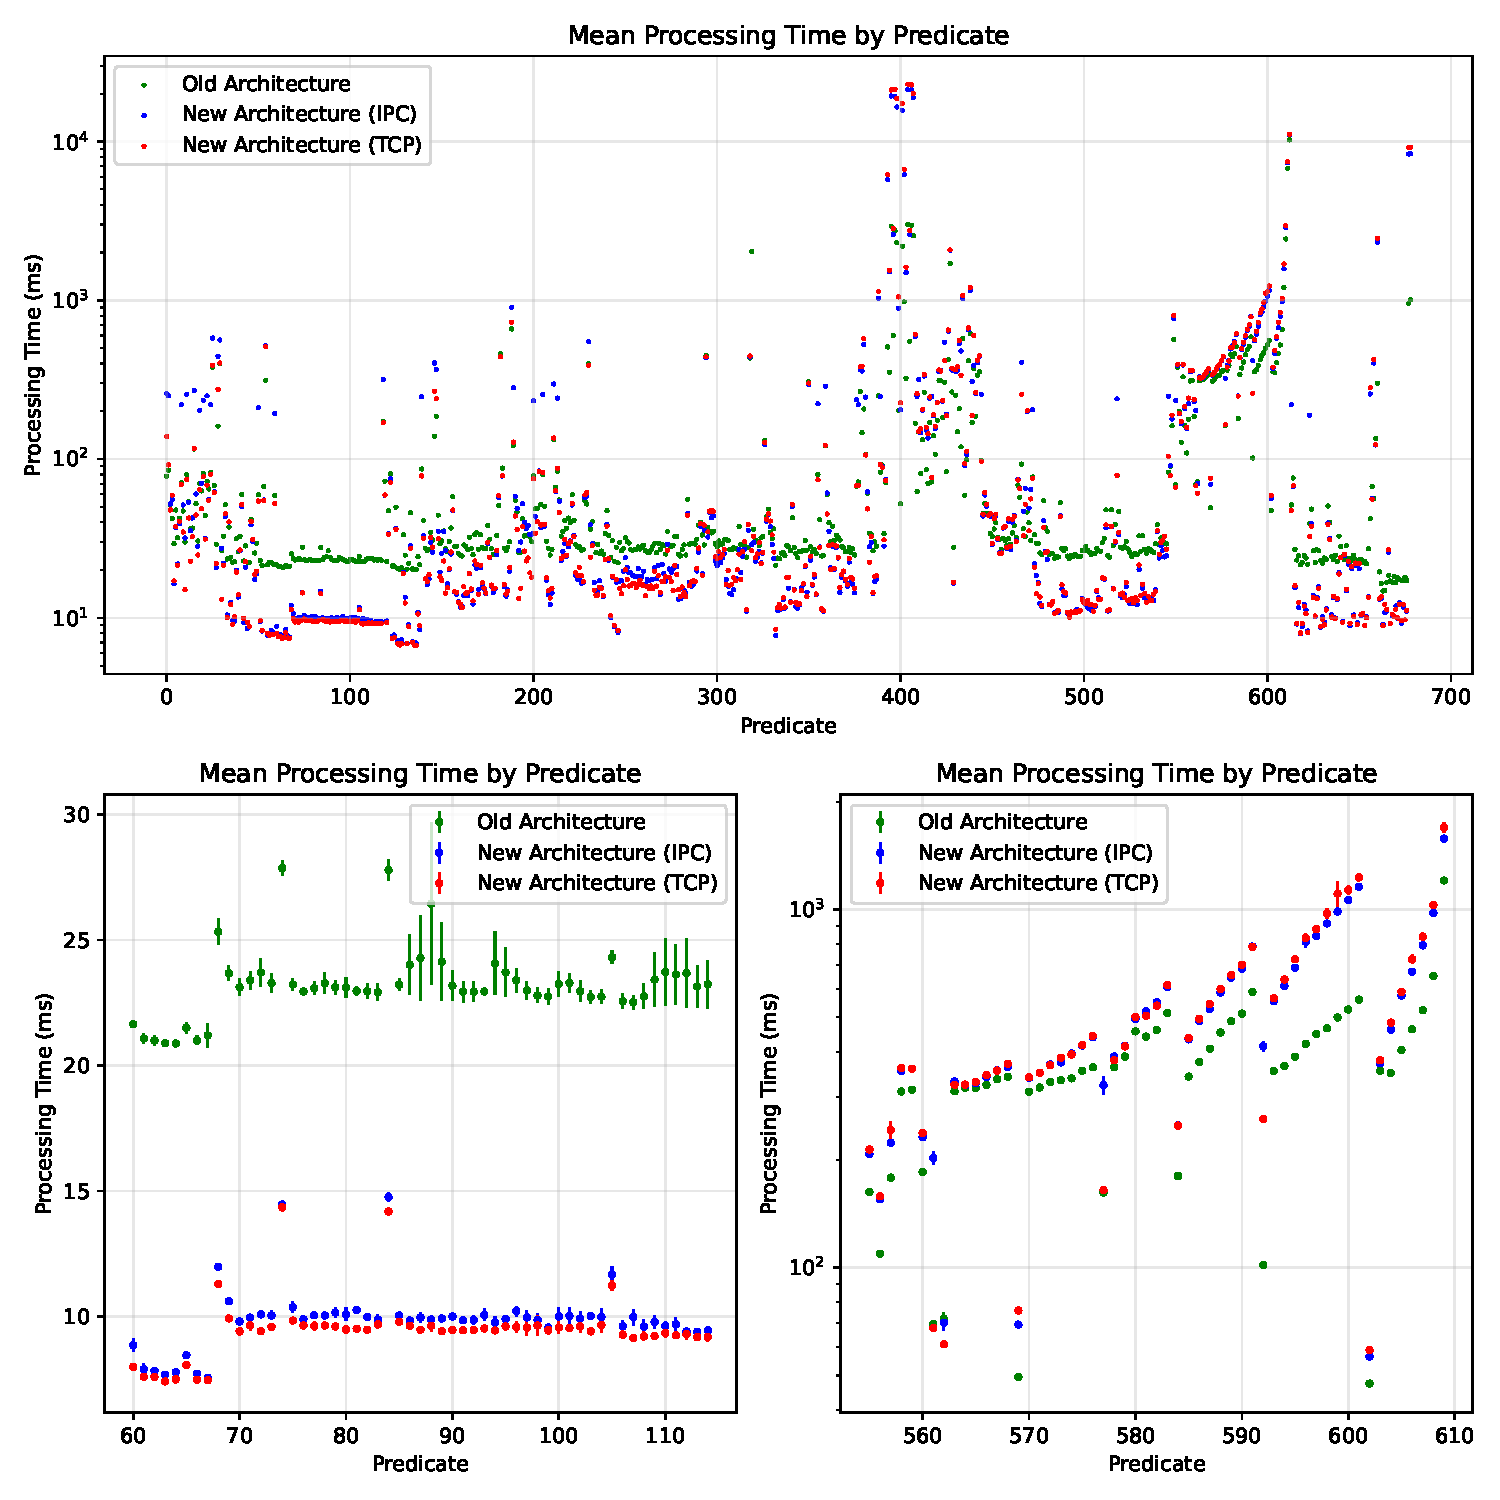
\includegraphics[scale=.55]{./PerformanceEvaluation/processingtime.pdf}
    \caption{Durchschnittliche Laufzeiten der Anfragen in den verschiedenen Architekturen.}
    \label{fig:performance-overview}
\end{figure}
% \FloatBarrier

Um sich zunächst einen Überblick über die Rohdaten zu verschaffen,
werden in \cref{fig:performance-overview} die durchschnittlichen Laufzeiten in den verschiedenen Konfigurationen dargestellt.
Der obere Subgraph zeigt die durchschnittlichen Laufzeiten aller Anfragen in sowohl der alten als auch der neuen Architektur,
wobei die neue Architektur in das IPC-Protokoll und TCP-Protokoll unterteilt ist.
Wider Erwarten zeigt sich, dass die durchschnittliche Laufzeit in der neuen Architektur bei vielen Prädikaten geringer ausfällt als in der alten Architektur.
Insgesamt sind von den 679 Prädikaten nur 172 Prädikate in der alten Architektur schneller gelöst worden.
265 Prädikate wurden in der IPC-Konfiguration und 242 Prädikate in der TCP-Konfiguration am schnellsten gelöst.

Die unteren beiden Subgraphen stellen interessante Bereiche der Rohdaten erneut dar und zeigen zusätzlich
die Standardfehler der Mittelwerte in Form der Fehlerbalken. Diese geben an, wie sehr die
Mittelwerte der Laufzeiten von den tatsächlichen Mittelwerten der Grundgesamtheit abweichen.
Kalkuliert wird dieser Standardfehler mittels der folgenden Formel:
\begin{equation}
    \sigma_{\overline{x}} = \frac{\sigma}{\sqrt{n}}
\end{equation}
Hierbei ist $\sigma_{\overline{x}}$ der Standardfehler des Mittelwertes, $\sigma$ die Standardabweichung der Grundgesamtheit und $n$ die Anzahl der Messungen.
Somit werden ausschließlich statistische Fehler betrachtet und systematische Fehler nicht berücksichtigt.

So zeigt der untere linke Subgraph die Rohdaten im Bereich der Prädikate 60 bis 115 erneut,
wobei klar zu erkennen ist, dass hier die neue Server-Architektur konstant schneller ist.
Dieser Trend ist über die gesamte Messung hin unterhalb einer gewissen Grenze zu beobachten.
Ebenfalls ersichtlich ist der nur minimal ausfallende Unterschied zwischen IPC und TCP.

Auf der anderen Seite zeigt der untere rechte Subgraph die Rohdaten im Bereich der Prädikate 555 bis 610.
Hier haben die Laufzeit Messungen einen vergleichsweise hohen Wert und es ist zu erkennen,
dass die alte Architektur in diesem Bereich schneller ist.

Entsprechend wurde durch die Protokollkommunikation ein Performance-Overhead eingeführt, der sich in den Rohdaten dahingehend widerspiegelt,
dass Prädikate, welche bereits eine hohe Laufzeit aufgewiesen haben, nun in der neuen Architektur noch langsamer gelöst werden.
Neben diesem Overhead wurde jedoch eine signifikante Laufzeitverbesserung erworben, die bis zu einer gewissen Gesamtlaufzeitsgrenze den
Overhead nicht nur annulliert, sondern überkompensiert.
Insgesamt scheint die neu eingeführte Server-Architektur hinsichtlich der Laufzeitperformance um einen gewissen Faktor effizienter geworden zu sein.

Ebenfalls ist zu erkennen, dass der Unterschied zwischen IPC und TCP nur minimal ist und keine signifikanten Unterschiede aufweist.
Innerhalb der 679 Testprädikaten ist IPC in 365 ($53.76\%$) Fällen schneller als TCP und entsprechend TCP in 314 ($46.24\%$) Fällen schneller als IPC.
Da zur TCP-Kommunikation die Adresse \texttt{tcp://127.0.0.1} verwendet wurde, ist eine mögliche Erklärung hierfür, dass die Kommunikation über das Loopback-Interface
einen Großteil des Netzwerk-Stacks umgeht und vom Betriebssystem speziell optimiert wird.
In der weiteren Analyse wird daher nur das IPC-Protokoll betrachtet.

% \clearpage

Um den Overhead der neuen Architektur zu quantifizieren,
wird die Differenz der durchschnittlichen Laufzeiten der neuen ($\overline{t_\text{IPC}}$) und alten ($\overline{t_\text{Old}}$) Architektur berechnet
und gegen die Anzahl der ZeroMQ-Anfragen analysiert.
Der induzierte Overhead $t_\text{induced}$ wird also wie folgt definiert:

\begin{equation}
    t_\text{induced} = \overline{t_\text{IPC}} - \overline{t_\text{Old}}
\end{equation}

Der oberste Subgraph in \cref{fig:overhead} zeigt den induzierten Overhead der neuen Architektur in Abhängigkeit der Anzahl der ZeroMQ-Anfragen auf einer logarithmischen Skala.
Im groben Verlauf ist zu erkennen, dass der Overhead mit steigender Anzahl der Anfragen annähernd linear zunimmt.
Zusätzlich scheint jedoch eine ausgeprägte Systematik vorzuliegen, welche sich inhaltlich durch die horizontale Verzerrung der Daten ausprägt.
Einige wenige Datenpunkte weichen stark von jeglicher Systematik ab und sind als Ausreißer zu klassifizieren.

Im zweiten Subgraphen wird die lineare Abhängigkeit des Overheads von der Anzahl der Anfragen untersucht, indem der Zusammenhang linear gefittet\footnote{Der lineare Fit wurde mit dem von scipi.optimize bereitgestellten curve\_fit berechnet.} wird.
Dies geschieht unter Berücksichtigung des kombinierten Standardfehlers der Mittelwerte der alten und neuen IPC-Architektur.
Die Unsicherheitsberechnung wird berechnet mit der gaußschen Fehlerfortpflanzung

\begin{equation}
    \sigma_{\overline{comb}} = \sqrt{\sigma_{\overline{IPC}}^2 + \sigma_{\overline{Old}}^2} \hspace{0.3cm},
\end{equation}

welche ebenfalls in den Fehlerbalken dargestellt wird.
Das Ergebnis des linearen Fits zeigt eine Steigung von $0.03 ms$ pro Anfrage, was bedeutet, dass der Overhead pro Anfrage um $0.03 ms$ steigt.
Zusätzlich gibt es einen y-Achsenabschnitt von $-13.13 ms$, was bedeutet, dass der Overhead bei $0$ Anfragen $-13.13 ms$ beträgt.
Dieser Wert beschreibt die zuvor erfasste Laufzeitverbesserung der neuen Architektur.
Insgesamt ergibt sich die folgende lineare Funktion zur Beschreibung des Overheads:

\begin{equation}
    Overhead = 0.03ms \cdot Anfragenanzahl - 13.13ms
\end{equation}

Durch das Kalkulieren der Nullstellen dieser Overhead-Funktion ergibt sich eine Anzahl an Anfragen von etwa $438$, bis der Overhead nicht länger von der Laufzeitverbesserung kompensiert werden kann.

Eine separate Messreihe wurde durchgeführt, um die durchschnittliche Laufzeit einer einzelnen Anfrage an den Z3-Server zu ermitteln.
Hierbei wurde die durchschnittliche Laufzeit von $0.0054 ms$ bestimmt.
Da für jede Anfrage zwei Nachrichten (Anfrage und Antwort) über den Socket gesendet werden, ergibt sich eine Laufzeit von $0.0216 ms$ pro Anfrage
unter der Annahme, dass das Erhalten einer ZeroMQ-Nachricht die gleiche Laufzeit aufweist wie das Senden einer Nachricht.
Die Differenz von $0.0084 ms$ zur ermittelten Steigung des linearen Fits könnte beispielsweise auf die Größe der Nachrichten zurückzuführen, welche
in der kontrollierten Messreihe einer einzelnen Anfrage kleiner ausfällt als in den 52 Testszenarien.
Zudem sind Messwerte dieser Größenordnung zunehmend ungenau, weshalb sie annehmbar plausibel bezüglich der Steigung des linearen Fits sind.


\begin{figure}[!htp]
    \centering
    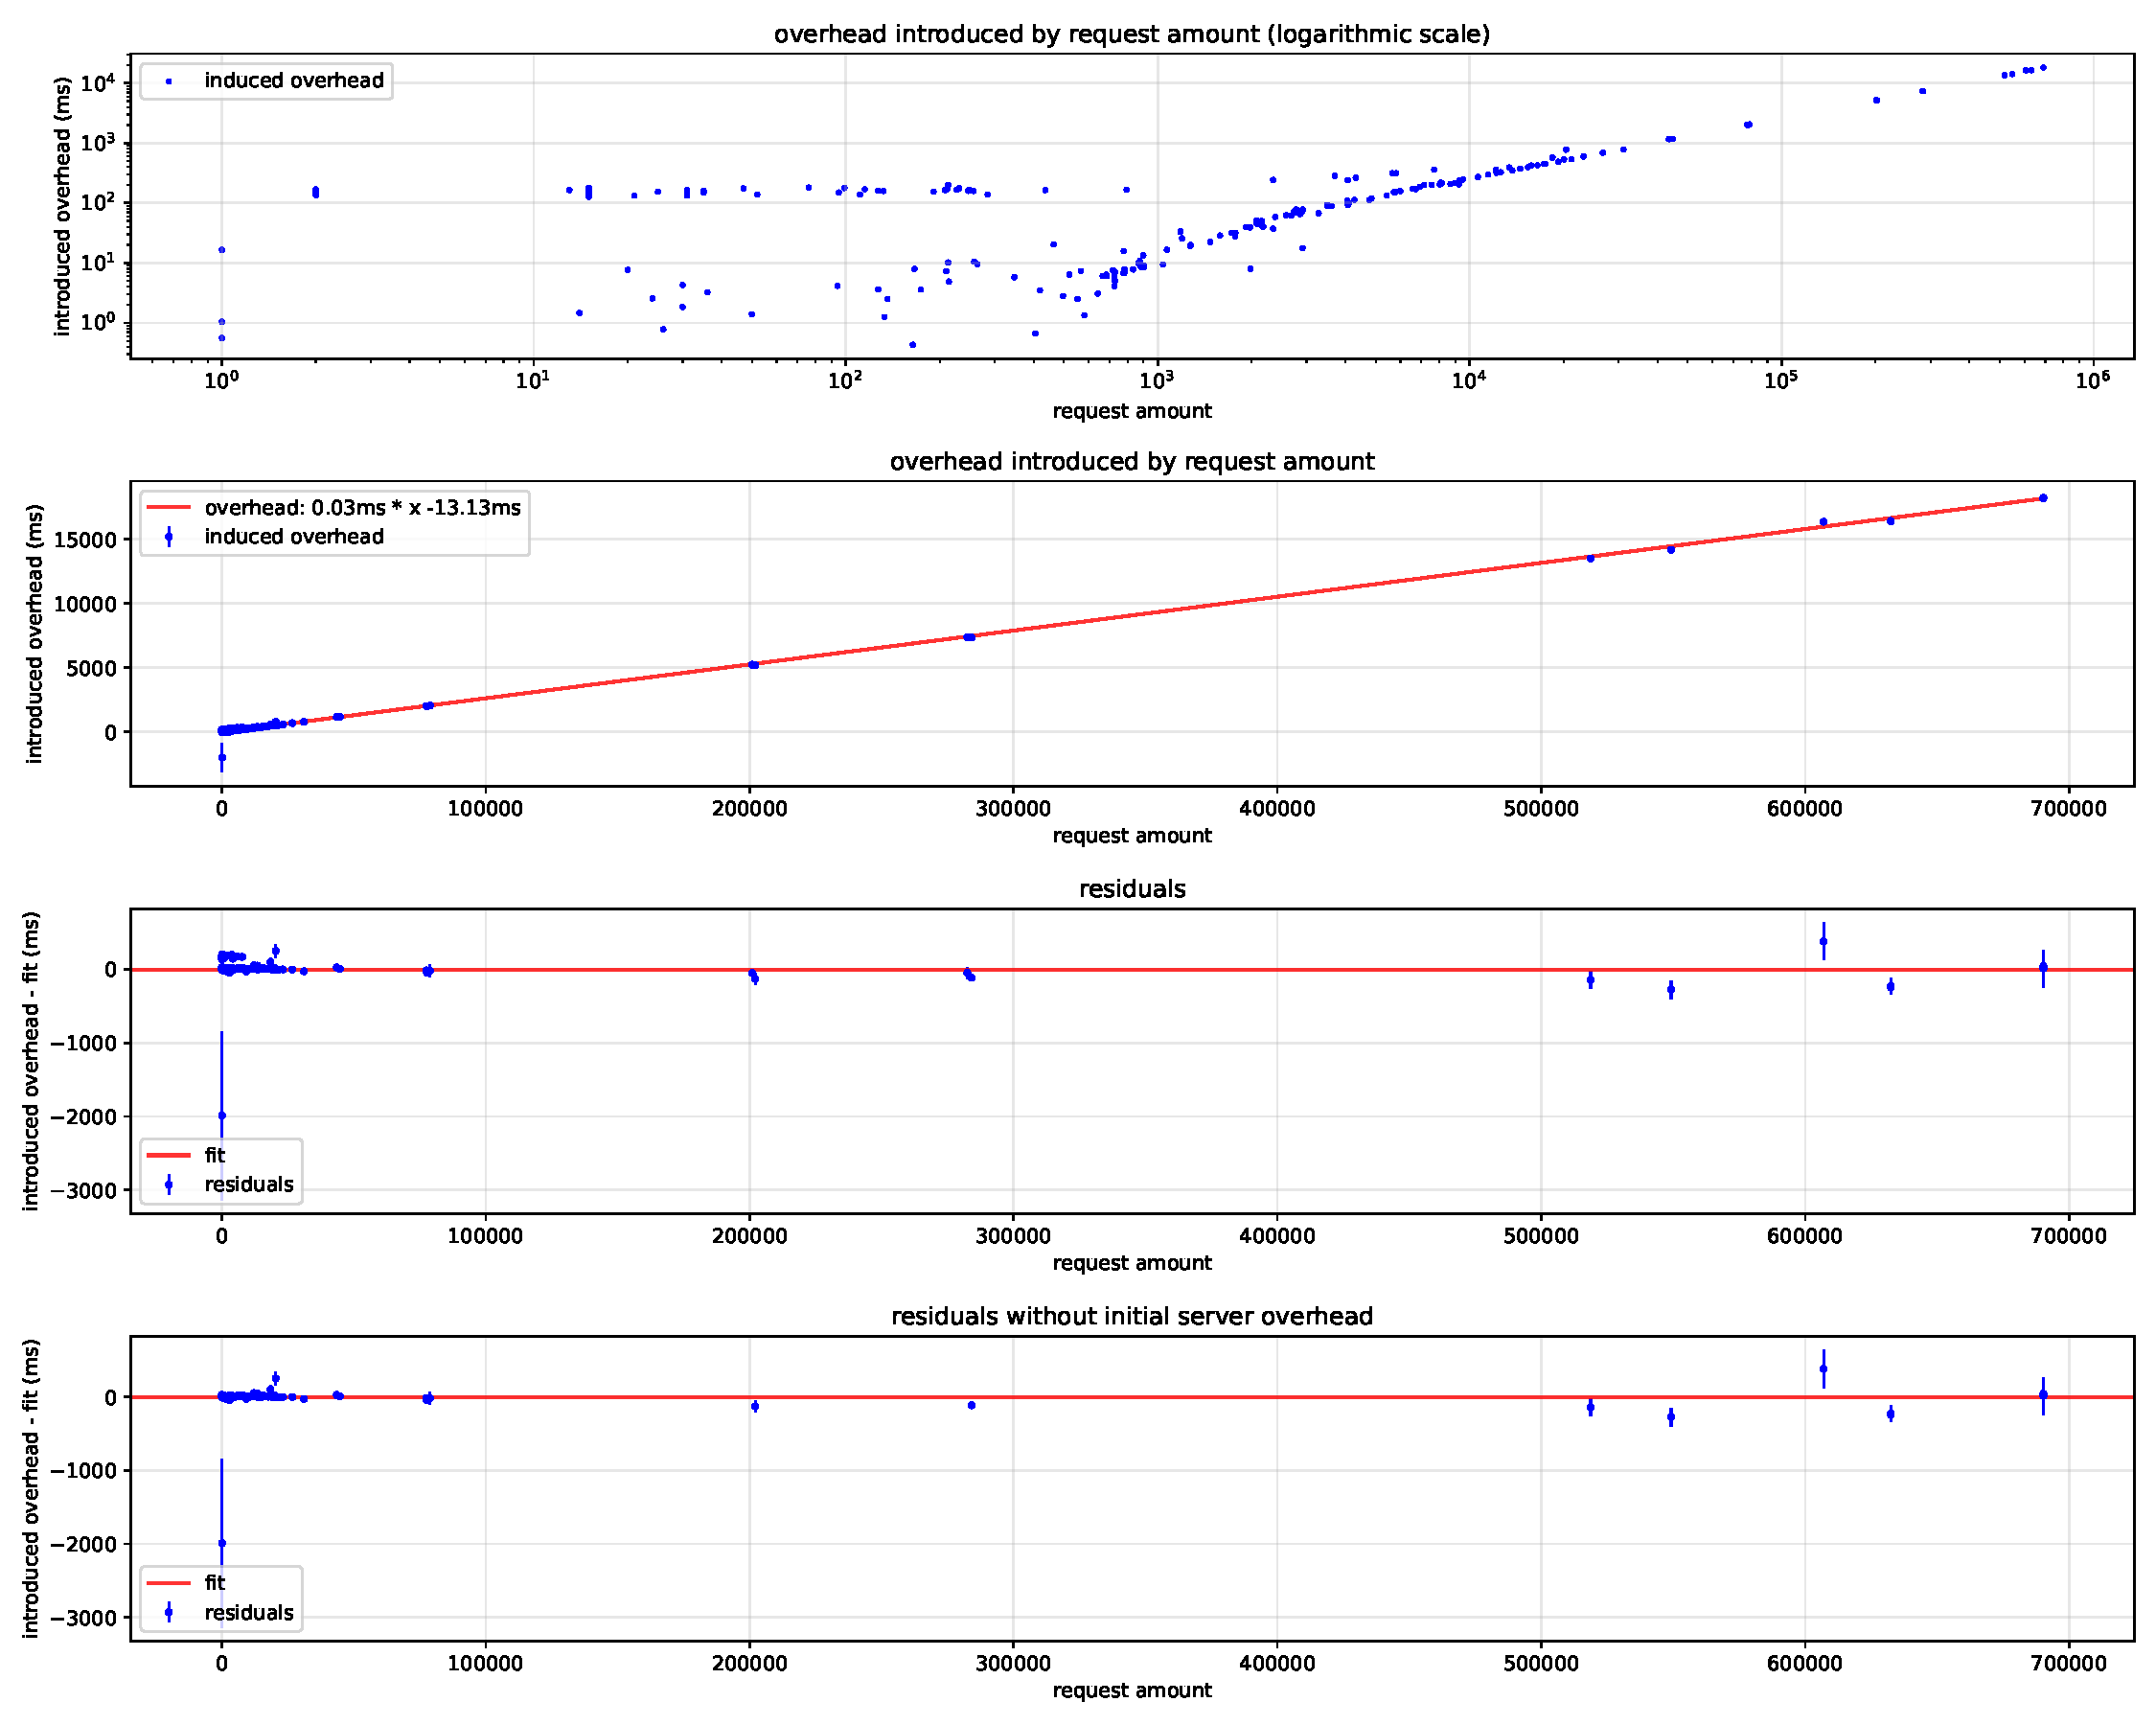
\includegraphics[scale=.55]{./PerformanceEvaluation/overhead.pdf}
    \caption{Induzierter Overhead der neuen Server-Architektur durch das Serialisieren auf den Socket.}
    \label{fig:overhead}
\end{figure}
% \FloatBarrier
% \clearpage

Der lineare Fit zeigt augenscheinlich eine gute Übereinstimmung mit den Daten, welche in dem dritten Subgraphen aus \cref{fig:overhead} verifiziert wird.
Hierbei wird die Differenz des induzierten Overheads und des linearen Fits gegen die Anzahl der Anfragen dargestellt.
Es ergibt sich ein Residuenplot.
In diesem Plot ist die Systematik des obersten Subgraphen erneut zu erkennen.
Sie bildet ein kleines Cluster oberhalb der $0$-Linie, bei sehr kleinen Anfragenzahlen.
Es stellt sich heraus, dass innerhalb dieses Datenclusters alle Datenpunkte die QueryID $1$ aufweisen.
Somit lässt sich die Abweichung durch das Initialisieren des Sockets, der Verbindung des Z3-Servers und dessen initialen Overheads zum Aufsetzten der Z3-Konfigurationen erklären.
Innerhalb einer TestID wird der Z3-Server nur einmalig initialisiert und folgende Prädikate desselben Tests nutzen denselben Z3-Server, indem sie die Konfiguration zurücksetzten und nicht grundlegend neu initialisieren.

Zur Überprüfung stellt der letzte Subgraph erneut den Residuenplot dar, jedoch ohne diejenigen Datenpunkte mit QueryID $1$.
Hierbei ist zu erkennen, dass die Systematik des vorherigen Graphen verschwindet und der lineare Fit eine gute Übereinstimmung mit den Daten aufweist.
Somit ist gezeigt, dass der Overhead der neuen Architektur durch das Serialisieren auf den Socket annähernd linear mit der Anzahl der Anfragen zunimmt
und keine weiteren relevanten Systematiken besitzt. Eine Voraussage des Overheads ist mithilfe des linearen Fits möglich.
Es ist zu beachten, dass die absoluten Werte des Overheads nur in der gegebenen Testumgebung gültig sind und nicht auf andere Umgebungen übertragen werden können.

Ein einzelner Datenpunkt scheint eine unwahrscheinlich hohe Laufzeitverbesserung von durchschnittlich $2$ Sekunden aufzuweisen, weist jedoch hohe Messunsicherheiten auf.
In \cref{tab:broken-datapoint} ist dieser Datenpunkt dargestellt.

\begin{table}[!htp]
    \centering
    \caption{Ausschnitt der gesammelten Messwerte eines Ausreißers.}
    \label{tab:broken-datapoint}
    \begin{tabular}{ cccccc }
        \toprule
        \textbf{TestID-QueryID} & \textbf{$Old_1(ms)$} & \textbf{$Old_2(ms)$} & \textbf{$Old_3(ms)$} & \textbf{$Old_4(ms)$} & \textbf{Req. Count} \\
        \midrule
        2122-90                 & 36                   & 4033                 & 3993                 & 43                   & 119                 \\
        \bottomrule
    \end{tabular}
\end{table}
% \FloatBarrier

Die verschiedenen Messwerte der alten Architektur in Millisekunden zeigen zwei starke Ausreißer bei der zweiten und dritten Messung.
Diese Varianz ist womöglich auf die in \cref{subsec:softlock} beschriebene Problematik zurückzuführen.
In jedem Fall ist dieser Datenpunkt als individueller Ausreißer zu betrachten und weist keine besondere statistische Relevanz auf.

Die ermittelte Performance-Verbesserung wird an dieser Stelle nicht weiter analysiert, da sie nicht Gegenstand dieser Arbeit ist.
Ein möglicher Grund für die Verbesserung könnte die Kompilierung sein, die durch die neue Architektur ermöglicht wird,
da der Z3-Solver als eigenständiger Prozess womöglich besser vom Compiler optimiert werden kann.
Als eigenständiger Prozess ist es ebenfalls möglich, dass der runtime linker die Z3-Bibliothek optimierter laden und ausführen kann.
Zusätzlich könnten die in \cref{subsec:optimizations} beschriebenen Optimierungen eine Rolle spielen.
